\documentclass[11pt,a4paper]{article}
\usepackage[margin=1in]{geometry}
\usepackage{hyperref}
\usepackage{xcolor}
\usepackage{tikz}
\usepackage{listings}
\usetikzlibrary{arrows.meta,positioning,shapes.multipart}

\hypersetup{
  colorlinks=true,
  linkcolor=blue,
  urlcolor=blue,
}

\lstdefinestyle{py}{
  language=Python,
  basicstyle=\ttfamily\small,
  keywordstyle=\color{blue!70!black},
  stringstyle=\color{green!40!black},
  commentstyle=\color{gray!60},
  showstringspaces=false,
  frame=single,
  framerule=0.3pt,
  breaklines=true
}

\title{Automated Testing \\ \& Logging in Python -- Advanced}
\author{Study Guide}
\date{\today}

\begin{document}
\maketitle

\section*{Pytest Advanced Cheat Sheet}
\begin{itemize}
  \item \textbf{Parametrize}: complex cases and ids.
\begin{lstlisting}[style=py]
@pytest.mark.parametrize("a,b,expected", [
    (6, 3, 2), (5, 2, 2.5)
], ids=["int", "float"])
def test_div(a,b,expected):
    assert a/b == expected
\end{lstlisting}
  \item \textbf{Markers}: \texttt{@pytest.mark.slow}, select via \texttt{-m slow}
  \item \textbf{Skip/XFail}: \texttt{@pytest.mark.skip}, \texttt{@pytest.mark.xfail}
  \item \textbf{Fixture scopes}: \texttt{function}, \texttt{class}, \texttt{module}, \texttt{session}
\begin{lstlisting}[style=py]
@pytest.fixture(scope="session")
def db_conn():
    yield connect()
    disconnect()
\end{lstlisting}
  \item \textbf{Autouse fixtures}: apply implicitly for setup like env vars.
  \item \textbf{Parallel runs}: \texttt{pytest -n auto} (requires \texttt{pytest-xdist}).
\end{itemize}

\section*{Pytest Execution Diagram}
\begin{center}
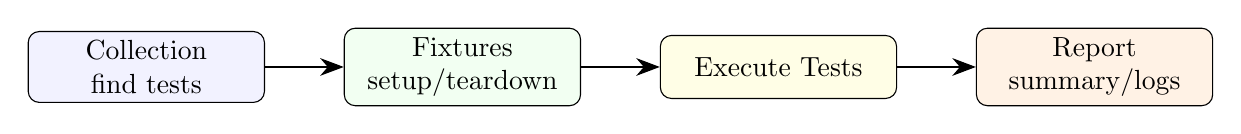
\begin{tikzpicture}[
  node distance=10mm,
  box/.style={draw, rounded corners, align=center, minimum width=30mm, minimum height=8mm},
  >={Stealth[length=3mm]}
]
  \node[box, fill=blue!5] (collect) {Collection\\find tests};
  \node[box, fill=green!5, right=of collect] (fixtures) {Fixtures\\setup/teardown};
  \node[box, fill=yellow!10, right=of fixtures] (execute) {Execute Tests};
  \node[box, fill=orange!10, right=of execute] (report) {Report\\summary/logs};
  \draw[->] (collect) -- (fixtures);
  \draw[->] (fixtures) -- (execute);
  \draw[->] (execute) -- (report);
\end{tikzpicture}
\end{center}

\section*{Logging Configuration (Production-Ready)}
Use \texttt{dictConfig} for structured, multi-handler logging.
\begin{lstlisting}[style=py]
import logging, logging.config

LOGGING = {
  "version": 1,
  "disable_existing_loggers": False,
  "formatters": {
    "std": {"format": "%(asctime)s [%(levelname)s] %(name)s: %(message)s"},
    "json": {"()": "pythonjsonlogger.jsonlogger.JsonFormatter"}
  },
  "handlers": {
    "console": {"class": "logging.StreamHandler", "formatter": "std"},
    "file": {
      "class": "logging.handlers.RotatingFileHandler",
      "filename": "app.log", "maxBytes": 1048576, "backupCount": 3,
      "formatter": "std"
    }
  },
  "root": {"level": "INFO", "handlers": ["console", "file"]}
}

logging.config.dictConfig(LOGGING)
logger = logging.getLogger(__name__)
logger.info("configured")
\end{lstlisting}

\textbf{Tip}: For JSON logs install \texttt{python-json-logger} and switch the formatter.

\section*{Pytest Logging Tips}
\begin{itemize}
  \item CLI live logs: \texttt{pytest -v --log-cli-level=INFO}
  \item Configure in \texttt{pytest.ini}:
\begin{lstlisting}
[pytest]
log_cli = true
log_cli_level = INFO
\end{lstlisting}
  \item Use \texttt{caplog.at\_level(level, logger=name)} for scoped capture.
\end{itemize}

\section*{Selenium Patterns (Advanced)}
\textbf{Page Object Model (POM)} skeleton:
\begin{lstlisting}[style=py]
from selenium.webdriver.common.by import By
from selenium.webdriver.support.ui import WebDriverWait
from selenium.webdriver.support import expected_conditions as EC

class LoginPage:
    URL = "https://www.saucedemo.com/"
    USER = (By.ID, "user-name")
    PASS = (By.ID, "password")
    BTN  = (By.ID, "login-button")

    def __init__(self, driver):
        self.driver = driver

    def open(self):
        self.driver.get(self.URL)

    def login(self, u, p):
        wait = WebDriverWait(self.driver, 10)
        wait.until(EC.visibility_of_element_located(self.USER)).send_keys(u)
        wait.until(EC.visibility_of_element_located(self.PASS)).send_keys(p)
        wait.until(EC.element_to_be_clickable(self.BTN)).click()
\end{lstlisting}

\textbf{Wait Strategies Cheat Sheet}
\begin{itemize}
  \item \texttt{visibility\_of\_element\_located}
  \item \texttt{element\_to\_be\_clickable}
  \item \texttt{presence\_of\_all\_elements\_located}
  \item \texttt{url\_contains} / \texttt{title\_contains}
\end{itemize}

\section*{Advanced Logging Diagram}
\begin{center}
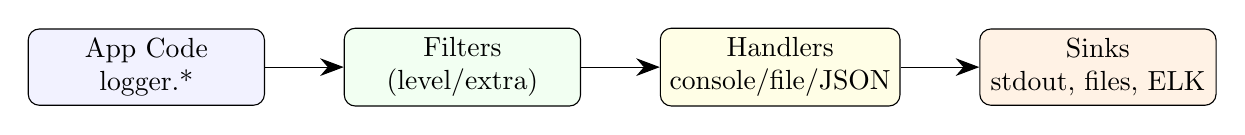
\begin{tikzpicture}[
  node distance=10mm,
  box/.style={draw, rounded corners, align=center, minimum width=30mm, minimum height=8mm},
  >={Stealth[length=3mm]}
]
  \node[box, fill=blue!5] (app) {App Code\\logger.*};
  \node[box, fill=green!5, right=of app] (filters) {Filters\\(level/extra)};
  \node[box, fill=yellow!10, right=of filters] (handlers) {Handlers\\console/file/JSON};
  \node[box, fill=orange!10, right=of handlers] (sinks) {Sinks\\stdout, files, ELK};
  \draw[->] (app) -- (filters);
  \draw[->] (filters) -- (handlers);
  \draw[->] (handlers) -- (sinks);
\end{tikzpicture}
\end{center}

\section*{Flaky Test Mitigation}
\begin{itemize}
  \item Replace \texttt{sleep} with explicit waits.
  \item Isolate state via \texttt{tmp\_path}/\texttt{monkeypatch}.
  \item Use retries sparingly (e.g., \texttt{flaky} or custom wrapper).
  \item Run in CI with deterministic seeds and timeouts.
\end{itemize}

\end{document}
